\hypertarget{introduction}{%
\section{Introduction}\label{introduction}}

Argument Mining (AM) is the automatic identification and extraction of
argumentative structures from natural language discourse {[}1{]}. In
order to achieve this, the discourse can first be segmented into
Elementary Discourse Units (EDUs), atomic units of the discourse. The
EDUs can then be classified into argument and non-argument, the
argumentative EDUs can be termed Argumentative Discourse Units (ADUs).
Following this, clausal properties can be determined for each ADU (e.g
for an ADU X, is X evidence? or is X a premise?). Finally, the relations
between ADUs can be determined (e.g.~does one ADU support or attack
another?). It is with this final step that this research is concerned.

The task of identifying the relational properties between already
identified ADUs is known as Argument Relation Identification (ARI). ARI
concerns itself both with identifying whether a relation exists between
to ADUs, and also classifying the type of relation, (typically either
support or attack). This typically becomes a 3-class classification
problem, concerning no relation, support and attack {[}2{]}.

There are, however, varying opinions on whether having only two
relational classes is enough, Inference Anchoring Theory (IAT) presents
three different classes {[}3{]}, {[}4{]}. In IAT, the `support' class is
split into `inference' or RA and `rephrase' or MA. The `attack' relation
is also termed `conflict' or CA. Using the IAT relation classes produces
a 4-class classification problem.

Transformer models {[}5{]} have significantly improved performance in
many tasks across natural language processing, including AM {[}6{]},
{[}7{]}. Subsequent task-agnostic pretraining approaches have allowed
these models to be fine-tuned on a wide variety of tasks. As the RoBERTa
model {[}8{]} has been shown to perform well in the ARI task {[}6{]} it
is used for this research to allow comparison with previous work.

Multimodal models have also proven useful in audio-based natural
language tasks, where transcripts of the spoken word are aso available.
Generally it has appeared that combining both audio and textual features
has seen improved performance over unimodal techniques {[}9{]},
{[}10{]}.

\hypertarget{datasets}{%
\section{Datasets}\label{datasets}}

All datasets used in this project are available as corpora on
AIFdb\footnote{https://corpora.aifdb.org/}. Using consistently annotated
Argument Interchange Format (AIF) data allows many different datasets to
be used and tested. The AIF Format {[}11{]} allows the annotation of
argument data across all AM tasks, providing a platform for many
different kinds of research.

\hypertarget{preprocessing}{%
\subsection{Preprocessing}\label{preprocessing}}

\hypertarget{argument-data}{%
\subsubsection{Argument Data}\label{argument-data}}

In order to use AIF data efficiently for ARI, it is useful to perform
some preprocessing. This process produces a graph, where each node
contains a locution, its related proposition, and the proposition's AIF
identifier. This identifier corresponds to the audio data, allowing it
to be easily loaded when required. Each edge in this graph corresponds
to a relation between the propositions, one of RA (inference), MA
(rephrase) or CA (conflict).

\begin{figure}[h!]
\begin{center}
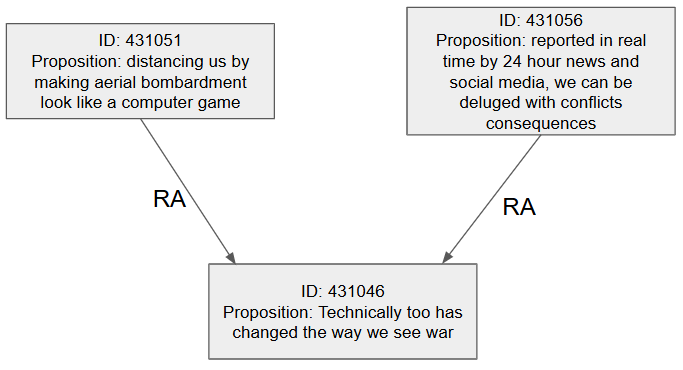
\includegraphics[width=10cm]{argument-map}
\caption{Example sub-graph \label{fig:arg-map}}
\end{center}
\end{figure}

Figure \ref{fig:arg-map} shows an example sub-graph from the larger
argument graph. Each node is truncated for brevity and only shows the
node's ID, and the proposition. This sub-graph is taken from the Moral
Maze episode on the 75th Anniversary of D-Day.

An example of the JSON structure used to store the argument data is
shown below.

\begin{Shaded}
\begin{Highlighting}[numbers=left,,]
\NormalTok{\{}
    \StringTok{"id"}\OperatorTok{:} \DecValTok{433407}\OperatorTok{,}
    \StringTok{"locution"}\OperatorTok{:} \StringTok{"Matthew Taylor : she answered questions about norms and structures by talking about beliefs and campaigns and I think beliefs are different to norms and I think campaigns are different to social structures"}\OperatorTok{,}
    \StringTok{"proposition"}\OperatorTok{:} \StringTok{"Nancy Sherman answered questions about norms and structures by talking about beliefs and campaigns and beliefs are different to norms and campaigns are different to social structures"}\OperatorTok{,}
    \StringTok{"relations"}\OperatorTok{:}\NormalTok{ [}
\NormalTok{        \{}
            \StringTok{"type"}\OperatorTok{:} \StringTok{"CA"}\OperatorTok{,}
            \StringTok{"to\_node\_id"}\OperatorTok{:} \DecValTok{433393}
\NormalTok{        \}}\OperatorTok{,}
\NormalTok{        \{}
            \StringTok{"type"}\OperatorTok{:} \StringTok{"RA"}\OperatorTok{,}
            \StringTok{"to\_node\_id"}\OperatorTok{:} \DecValTok{433416}
\NormalTok{        \}}
\NormalTok{    ]}\OperatorTok{,}
\NormalTok{\}}
\end{Highlighting}
\end{Shaded}

\hypertarget{audio-data}{%
\subsubsection{Audio Data}\label{audio-data}}

\hypertarget{qt30}{%
\subsection{QT30}\label{qt30}}

\hypertarget{moral-maze}{%
\subsection{Moral Maze}\label{moral-maze}}

\hypertarget{models}{%
\section{Models}\label{models}}

\hypertarget{preliminary-results}{%
\section{Preliminary Results}\label{preliminary-results}}

\hypertarget{conclusion}{%
\section{Conclusion}\label{conclusion}}

\hypertarget{references}{%
\section*{References}\label{references}}
\addcontentsline{toc}{section}{References}

\hypertarget{refs}{}
\begin{CSLReferences}{0}{0}
\leavevmode\vadjust pre{\hypertarget{ref-lawrenceArgumentMiningSurvey2020}{}}%
\CSLLeftMargin{{[}1{]} }%
\CSLRightInline{J. Lawrence and C. Reed, {``Argument {Mining}: {A
Survey},''} \emph{Computational Linguistics}, vol. 45, no. 4, pp.
765--818, Jan. 2020, doi:
\href{https://doi.org/10.1162/coli_a_00364}{10.1162/coli\_a\_00364}.}

\leavevmode\vadjust pre{\hypertarget{ref-gemechuARIESGeneralBenchmark2024}{}}%
\CSLLeftMargin{{[}2{]} }%
\CSLRightInline{D. Gemechu, R. Ruiz-Dolz, and C. Reed, {``{ARIES}: {A
General Benchmark} for {Argument Relation Identification},''} in
\emph{Proceedings of the 11th {Workshop} on {Argument Mining}
({ArgMining} 2024)}, Aug. 2024, pp. 1--14. doi:
\href{https://doi.org/10.18653/v1/2024.argmining-1.1}{10.18653/v1/2024.argmining-1.1}.}

\leavevmode\vadjust pre{\hypertarget{ref-budzynskaArgumentMiningDialogue2014}{}}%
\CSLLeftMargin{{[}3{]} }%
\CSLRightInline{K. Budzynska \emph{et al.}, {``Towards {Argument Mining}
from {Dialogue},''} in \emph{Computational {Models} of {Argument}}, IOS
Press, 2014, pp. 185--196. doi:
\href{https://doi.org/10.3233/978-1-61499-436-7-185}{10.3233/978-1-61499-436-7-185}.}

\leavevmode\vadjust pre{\hypertarget{ref-budzynskaModelProcessingIllocutionary2014}{}}%
\CSLLeftMargin{{[}4{]} }%
\CSLRightInline{K. Budzynska, M. Janier, C. Reed, P. Saint-Dizier, M.
Stede, and O. Yakorska, {``A {Model} for {Processing Illocutionary
Structures} and {Argumentation} in {Debates},''} in \emph{Proceedings of
the {Ninth International Conference} on {Language Resources} and
{Evaluation} ({LREC}`14)}, May 2014, pp. 917--924.}

\leavevmode\vadjust pre{\hypertarget{ref-vaswaniAttentionAllYou2017}{}}%
\CSLLeftMargin{{[}5{]} }%
\CSLRightInline{A. Vaswani \emph{et al.}, {``Attention {Is All You
Need},''} p. 11, 2017.}

\leavevmode\vadjust pre{\hypertarget{ref-ruiz-dolzTransformerBasedModelsAutomatic2021}{}}%
\CSLLeftMargin{{[}6{]} }%
\CSLRightInline{R. Ruiz-Dolz, J. Alemany, S. M. H. Barberá, and A.
García-Fornes, {``Transformer-{Based Models} for {Automatic
Identification} of {Argument Relations}: {A Cross-Domain Evaluation},''}
\emph{IEEE Intelligent Systems}, vol. 36, no. 6, pp. 62--70, Nov. 2021,
doi:
\href{https://doi.org/10.1109/MIS.2021.3073993}{10.1109/MIS.2021.3073993}.}

\leavevmode\vadjust pre{\hypertarget{ref-wuKnowCompDialAM2024Finetuning2024}{}}%
\CSLLeftMargin{{[}7{]} }%
\CSLRightInline{Y. Wu, Y. Zhou, B. Xu, W. Wang, and Y. Song,
{``{KnowComp} at {DialAM-2024}: {Fine-tuning Pre-trained Language
Models} for {Dialogical Argument Mining} with {Inference Anchoring
Theory},''} in \emph{Proceedings of the 11th {Workshop} on {Argument
Mining} ({ArgMining} 2024)}, Aug. 2024, pp. 103--109. doi:
\href{https://doi.org/10.18653/v1/2024.argmining-1.10}{10.18653/v1/2024.argmining-1.10}.}

\leavevmode\vadjust pre{\hypertarget{ref-liuRoBERTaRobustlyOptimized2019a}{}}%
\CSLLeftMargin{{[}8{]} }%
\CSLRightInline{Y. Liu \emph{et al.}, {``{RoBERTa}: {A Robustly
Optimized BERT Pretraining Approach}.''} arXiv, Jul. 2019. doi:
\href{https://doi.org/10.48550/arXiv.1907.11692}{10.48550/arXiv.1907.11692}.}

\leavevmode\vadjust pre{\hypertarget{ref-manciniMultimodalArgumentMining2022}{}}%
\CSLLeftMargin{{[}9{]} }%
\CSLRightInline{E. Mancini, F. Ruggeri, A. Galassi, and P. Torroni,
{``Multimodal {Argument Mining}: {A Case Study} in {Political
Debates},''} in \emph{Proceedings of the 9th {Workshop} on {Argument
Mining}}, Oct. 2022, pp. 158--170.}

\leavevmode\vadjust pre{\hypertarget{ref-manciniMAMKitComprehensiveMultimodal2024}{}}%
\CSLLeftMargin{{[}10{]} }%
\CSLRightInline{E. Mancini, F. Ruggeri, S. Colamonaco, A. Zecca, S.
Marro, and P. Torroni, {``{MAMKit}: {A Comprehensive Multimodal Argument
Mining Toolkit},''} in \emph{Proceedings of the 11th {Workshop} on
{Argument Mining} ({ArgMining} 2024)}, Aug. 2024, pp. 69--82. doi:
\href{https://doi.org/10.18653/v1/2024.argmining-1.7}{10.18653/v1/2024.argmining-1.7}.}

\leavevmode\vadjust pre{\hypertarget{ref-chesnevarArgumentInterchangeFormat2006}{}}%
\CSLLeftMargin{{[}11{]} }%
\CSLRightInline{C. Chesñevar \emph{et al.}, {``Towards an argument
interchange format,''} \emph{The Knowledge Engineering Review}, vol. 21,
no. 4, pp. 293--316, Dec. 2006, doi:
\href{https://doi.org/10.1017/S0269888906001044}{10.1017/S0269888906001044}.}

\end{CSLReferences}
